\chapter{栈和队列}

栈(stack)只能在表的一端插入和删除,先进后出(LIFO, Last In, First Out)。

队列(queue)只能在表的一端(队尾rear)插入,另一端(队头front)删除,先进先出(FIFO, First In, First Out)。

\section{栈} %%%%%%%%%%%%%%%%%%%%%%%%%%%%%%

\subsection{Hanoi塔问题}

\textbf{n阶Hanoi塔问题} 假设有三个分别命名为X、Y和Z的塔座,在塔座X上插有n个
直径大小各不相同、从小到大编号为1,2,...,n的圆盘,如图~\ref{fig:hanoiTower}所示。

\begin{center}
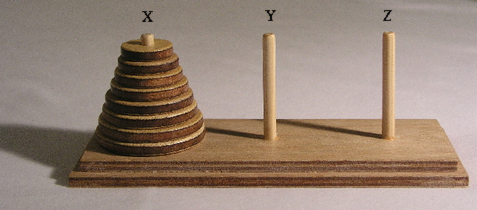
\includegraphics[width=180pt]{Tower-of-Hanoi.png}\\
\figcaption{Hanoi塔问题}\label{fig:hanoiTower}
\end{center}


现要求将X塔上的n个圆盘移动到Z上并仍按同样的顺序叠放,圆盘移动时必须遵循下列规则:
\begindot
\item 每次只能移动一个圆盘;
\item 圆盘可以插在X、Y和Z中的任一塔座上;
\item 任何时刻都不能将一个较大的圆盘压在较小的圆盘之上。
\myenddot

递归代码如下:
\begin{Codex}[label=hanoi.c]
/*
 * @brief 将塔座x上按直径有小到大且自上而下编号
 * 为1至n的n个圆盘按规则搬到塔座z上,y可用做辅助塔座.
 * @param[in] n 圆盘个数
 * @param[in] x 源塔座
 * @param[in] y 辅助塔座
 * @param[in] z 目标塔座
 * @return 无
 * @note 无
 * @remarks 无
 */
static void hanoi(int n, char x, char y, char z)
{
    if(n ==  1) {
        /* 移动操作move(x,n,z)可定义为(c是初始值为的全局
           变量,对搬动计数):
           printf("%i. Move disk %i from %c to %c\n",
                                        ++c, n, x, z);
        */
        move(1, x, z); /* 将编号为1的圆盘从x移动到z */
        return;
    } else {
        /* 将x上编号1至n-1的圆盘移到y,z作辅助塔*/
        hanoi(n-1, x, z, y); 
        move(n,x,z);  /* 将编号为n的圆盘从x移到z */
        /* 将y上编号至n-1的圆盘移到z,x作辅助塔*/
        hanoi(n-1, y, x, z); 
    }
}
\end{Codex}

\subsection{数制转换}
\begin{Codex}[label=convert_base.cpp]
 /*
  * @brief 数制转换,将一个整数转化为 d进制,d<=16.
  * @param[in] n 整数n
  * @param[in] d d进制
  * @return 无
  */
static void convert_base(int n, const int d)
{
	std::stack<int> s;
	int e;

	while(n != 0) {
		e = n % d;
		s.push(e);
		n /= d;
	}
	while(!s.empty()) {
		e = s.top();
		s.pop();
		printf("%x", e);
	}
	return;
}

#define MAX 64 // 栈的最大长度
static int stack[MAX];
static int top = -1;
 /*
  * @brief 数制转换,将一个整数转化为 d进制,d<=16,更优化的版本.
  *
  * 如果可以预估栈的最大空间,则用数组来模拟栈,这时常用的一个技巧。
  * 这里,栈的最大长度是多少?假设CPU是64位,最大的整数则是2^64,由于
  * 数制最小为2,在这个进制下,数的位数最长,这就是栈的最大长度,最长为64。
  *
  * @param[in] n 整数n
  * @param[in] d d进制
  * @return 无
  */
static void convert_base2(int n, const int d)
{
	int e;

	while(n != 0) {
		e = n % d;
		stack[++top] = e; // push
		n /= d;
	}
	while(top >= 0) {
		e = stack[top--]; // pop
		printf("%x", e);
	}
	return;
}
\end{Codex}

\section{队列} %%%%%%%%%%%%%%%%%%%%%%%%%%%%%%

\subsection{打印杨辉三角}

\begin{Codex}[label=yanghui_triangle.cpp]
#include <queue>
/**
 * @brief 打印杨辉三角系数.
 *
 * 分行打印二项式(a+b)^n展开式的系数。在输出上一行
 * 系数的同时,将其下一行的系数预先计算好,放入队列中。
 * 在各行系数之间插入一个0。
 *
 * @param[in] n (a+b)^n
 * @return 无
 */
void yanghui_triangle(const int n)
{
    int i = 1;
    std::queue<int> q;
    /* 预先放入第一行的1 */
    q.push(i);

    for(i = 0; i <= n; i++) {	 /* 逐行处理*/
        int j;
        int s = 0;
        q.push(s);      /* 在各行间插入一个0*/

        /* 处理第i行的i+2个系数(包括一个0)*/
        for(j = 0; j < i+2; j++) {
            int t;
            int tmp;
            t = q.front();  /*读取一个系数,放入t*/
            q.pop();
            tmp = s + t;      /* 计算下一行系数,并进队列*/
            q.push(tmp);
            s = t;            /* 打印一个系数,第i+2个是0*/
            if(j != i+1) {
                printf("%d ",s);    
            }
        }
        printf("\n"); 
    }
}
\end{Codex}
